\documentclass[
	12pt,				% tamanho da fonte
	oneside,			% para impressão em recto e verso. Oposto a oneside
	a4paper,			% tamanho do papel. 
	english,			% idioma adicional para hifenização
	brazil,				% o último idioma é o principal do documento
	]{abntex2}

% ---
% Pacotes fundamentais 
% ---
\usepackage{lmodern}			% Usa a fonte Latin Modern
\usepackage[T1]{fontenc}		% Selecao de codigos de fonte.
\usepackage[utf8]{inputenc}		% Codificacao do documento (conversão automática dos acentos)
\usepackage{indentfirst}		% Indenta o primeiro parágrafo de cada seção.
\usepackage{color}				% Controle das cores
\usepackage{graphicx}			% Inclusão de gráficos
\usepackage{microtype} 			% para melhorias de justificação
\usepackage{multicol}
\usepackage{multirow}
\usepackage[brazilian,hyperpageref]{backref}	 % Paginas com as citações na bibl
\usepackage[alf]{abntex2cite}	% Citações padrão ABNT
\usepackage{listings}

\lstset{language=Java,
  showspaces=false,
  showtabs=false,
  breaklines=true,
  showstringspaces=false,
  breakatwhitespace=true,
  commentstyle=\color{green},
  keywordstyle=\color{blue},
  stringstyle=\color{red},
  basicstyle=\ttfamily
}

% --- 
% CONFIGURAÇÕES DE PACOTES
% --- 

% ---
% Configurações do pacote backref
% Usado sem a opção hyperpageref de backref
\renewcommand{\backrefpagesname}{Citado na(s) página(s):~}
% Texto padrão antes do número das páginas
\renewcommand{\backref}{}
% Define os textos da citação
\renewcommand*{\backrefalt}[4]{
	\ifcase #1 %
		Nenhuma citação no texto.%
	\or
		Citado na página #2.%
	\else
		Citado #1 vezes nas páginas #2.%
	\fi}%
% ---

% ---
% Informações de dados para CAPA e FOLHA DE ROSTO
% ---
\titulo{Prática 3, Conversor de Unidades de Medida}
\autor{Pedro Inácio Rodrigues Pontes}
\local{Belo Horizonte, Brasil}
\data{2025}
\instituicao{%
  Universidade Federal de Minas Gerais
  \par
  Colégio Técnico
  \par
  Curso Técnico em Desenvolvimento de Sistemas}

\definecolor{blue}{RGB}{41,5,195}

\makeatletter
\hypersetup{
     	%pagebackref=true,
		pdftitle={\@title}, 
		pdfauthor={\@author},
    	pdfsubject={\imprimirpreambulo},
		colorlinks=true,       		% false: boxed links; true: colored links
    	linkcolor=blue,          	% color of internal links
    	citecolor=blue,        		% color of links to bibliography
    	filecolor=magenta,      		% color of file links
		urlcolor=blue,
		bookmarksdepth=4
}
\makeatother

\renewcommand{\thesection}{\arabic{section}}
\setlength{\parindent}{1.3cm}
\setlength{\parskip}{0.2cm} 

\makeindex


\begin{document}

\selectlanguage{brazil}
\frenchspacing 

\imprimircapa

{
\ABNTEXchapterfont

\textual

% ----------------------------------------------------------
% Introdução (exemplo de capítulo sem numeração, mas presente no Sumário)
% ----------------------------------------------------------
\section{Introdução}

O objetivo da presente prática foi produzir um conversor de unidades de medida em C\# utilizando da interface gráfica Avalonia UI. Aqui estão os requerimentos para a interface:

\begin{enumerate}
    \item Permitir a seleção do tipo de conversão através de um ListBox
    \item Ter um campo de entrada para o valor de origem
    \item Ter um campo de saída para o valor convertido
    \item Incluir um botão para executar a conversão
    \item Tipos de Conversão e Fórmulas
\end{enumerate}

\section{Desenvolvimento}

Para conseguir alcançar o objetivo da confecção do conversor de unidades de medida, o projeto foi dividido utilizando o padrão MVVM (Model-View-ViewModel). View define a interface do usuário, onde é utilizado o código .xaml do avalonia, Model define as estruturas de dados da aplicação, ViewModel conecta os dois.

\subsection{Model}

Para a seção model, foi criada a classe ConversionType, a qual define a estrutura básica de uma conversão, que tem nome e sua fórmula, que foi representada utilizando uma \textit{Delgate Property}, a qual consiste em uma propriedade de classe que representa uma função que recebe um valor de parâmetro e devolve outro.

\begin{verbatim}
namespace ConversorDeUnidadesDeMedida.Models
{
    public class ConversionType
    {
        public string Name { get; set; }
        public Func<double, double> ConversionFormula { get; set; }

        public ConversionType(string name, Func<double, double> conversionFormula)
        {
            Name = name;
            ConversionFormula = conversionFormula;
        }
    }
}
\end{verbatim}

\subsection{Services}

Além da divisão base do modelo MVVM, foi adicionado também o modelo Services, onde se encontra o ConversionService, o qual retorna uma lista com todos os tipos de conversão:

\begin{verbatim}
namespace ConversorDeUnidadesDeMedida.Services
{
    public static class ConversionService
    {
        public static List<ConversionType> GetConversionTypes()
        {
            return new List<ConversionType>
            {
                new ConversionType("Celsius para Fahrenheit", c => (c * 1.8) + 32),
                new ConversionType("Fahrenheit para Celsius", f => (f - 32) / 1.8),
                new ConversionType("Celsius para Kelvin", c => c + 273.15),
                new ConversionType("Kelvin para Celsius", k => k - 273.15),
                new ConversionType("Metros para Pés", m => m * 3.28084),
                new ConversionType("Pés para Metros", ft => ft * 0.3048),
                new ConversionType("Quilômetros para Milhas", km => km * 0.621371),
                new ConversionType("Milhas para Quilômetros", mi => mi * 1.60934),
                new ConversionType("Quilogramas para Libras", kg => kg * 2.20462),
                new ConversionType("Libras para Quilogramas", lb => lb * 0.453592),
                new ConversionType("Gramas para Onças", g => g * 0.035274),
                new ConversionType("Onças para Gramas", oz => oz * 28.3495),
                new ConversionType("Litros para Galões", l => l * 0.264172),
                new ConversionType("Galões para Litros", gal => gal * 3.78541),
                new ConversionType("Mililitros para Onças Fluidas", ml => ml * 0.033814),
                new ConversionType("Onças Fluidas para Mililitros", flOz => flOz * 29.5735)
            };
        }
    }
}
\end{verbatim}

\subsection{View}
 
Para o modelo View, representado principalmente por MainWindow.axaml, foram utilizados os tipos ListBox para fazer a lista de conversões, TextBox para receber e exibir os valores e Button para criar um botão para conversão, além do TextBloc para representar um bloco comum de texto. Segue a parte relevante do código:

\begin{verbatim}
<ListBox ItemsSource="{Binding ConversionTypes}" SelectedItem="{Binding SelectedConversionType}" 
         Grid.Row="0" Grid.Column="1" Margin="10" Height="100">
    <ListBox.ItemTemplate>
        <DataTemplate>
            <TextBlock Text="{Binding Name}" />
        </DataTemplate>
    </ListBox.ItemTemplate>
</ListBox>
[...]
<TextBox Text="{Binding InputValue}" Grid.Row="1" Grid.Column="1" Margin="10"/>
[...]
<TextBox Text="{Binding OutputValue}" Grid.Row="2"
Grid.Column="1" Margin="10" IsReadOnly="True"/>
[...]
<Button Content="Converter" Command="{Binding ConvertCommand}" Grid.Row="3"
Grid.Column="1" Margin="10" HorizontalAlignment="Right"/>
\end{verbatim}
Observa-se principalmente a Palavra \textit{Binding} dentro de chaves. Isso ocorre para chamar elementos da divisão ViewModel, que serão conectados automaticamente a elas, como ConvertCommand e Name. Essa funcionalidade do Avalonia é extremamente útil para separar as lógicas de View e backend.

\subsection{ViewModel}


\section{Resultados}

Todos os resultados foram alcançados perfeitamente, com a única ressalva de aparentemente o método Dump permitir a exibição de máximas 16 linhas de toda a seleção.



\begin{figure}[h]
    \centering
    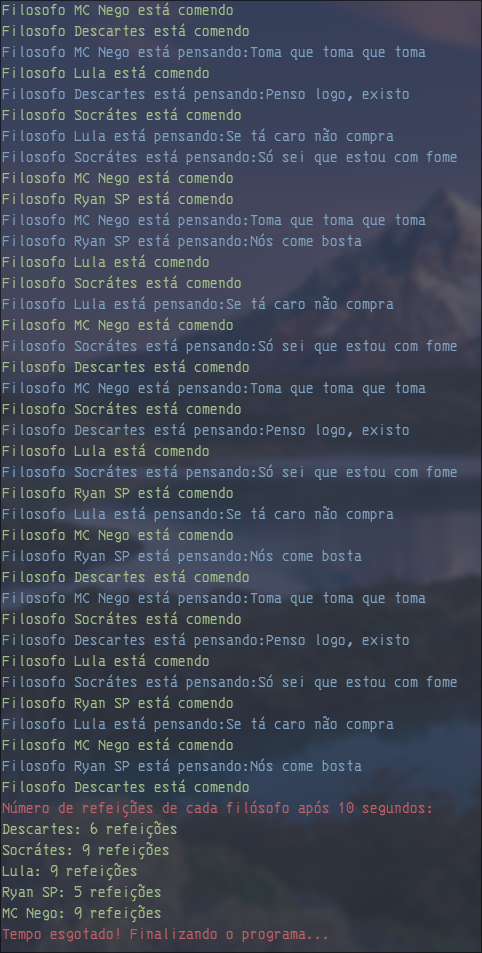
\includegraphics[width=0.7\textwidth]{img1.png}
    \caption{Resultado do Exércicio 10}
    \label{fig:img1}
\end{figure}

\section{Conclusão}

Todos os objetivos foram alcançados com sucesso. Os maiores problemas foram o método Dump não exibir mais de 16 linhas e a necessidade do uso do simbólo ? após alguns valores para permitir valores \textit{null}, e ?? para manipular um valor que será utilizado quando algum for \textit{null}. Outra observação é que o uso de LINQ lembra enormemente ao SQL.

\end{document}
